%This is the first chapter of the dissertation

%The following command starts your chapter. If you want different titles used in your ToC and at the top of the page throughout the chapter, you can specify those values here. Since Columbia doesn't want extra information in the headers and footers, the "Top of Page Title" value won't actually appear.

\chapter[The ATLAS detector][Top of Page Title]{The ATLAS detector} \label{Chapter-ATLAS}

The dataset analyzed in this thesis was taken by the ATLAS detector ~\cite{PERF-2007-01}, which is located at the ``Point 1'' cavern of the LHC, just across the street from the main CERN campus.
The much-maligned acronym stands for \textit{A} \textit{T}oriodal \textit{L}HC \textit{A}pparatu\textit{S}.
ATLAS is a massive cylindrical detector, with a radius of 12.5 m and a length of 44 m, with nearly hermetic coverage around the collision point.
Each of the many subdetectors plays a role in  measuring the energy, momentum, and type of the particles produced in collisions delivered by the LHC.
These subdetectors are immersed in a hybrid solenoid-toroid magnet system which allows for precise measurements of particle momenta.
The central solenoid magnet contains a magnetic field of $2$ T.
A schematic of the detector is shown in \Cref{fig:atlas_full}.

The \textit{inner detector} (ID) lies closest to the collision point, and contains three separate subdetectors.
It provides pseudorapidity\footnotemark coverage of $|\eta| < 2.5$ for charged particles.
\footnotetext{ATLAS uses a right-handed Cartesian coordinate system.
The origin is defined by the nominal beam interaction point.
The positive-$z$ direction is defined by the incoming beam travelling counterclockwise around the LHC.
The positive-$x$ direction points towards the center of the LHC ring from the origin, and the positive-$y$ direction points upwards towards the sky.
For particles of transverse (in the $x-y$ plane) momentum $p_T = \sqrt{p_x^2 + p_y^2}$ and energy $E$, it is generally most convenient fully describe this particle's kinematics as measured by the detector in the $(p_T, \phi, \eta, E)$ basis.
The angle $\phi = \arctan(p_y/p_x)$ is the standard azimuthal angle, and $\eta = \ln{\tan(\theta/2)} $ is known as the pseudorapidity, and defined based on the standard polar angle $\theta = \arccos(p_z/p_T)$.
For locations of detector elements, both $(r, \phi, \eta)$ and $(z, \phi, \eta)$ can be useful.}
The tracks reconstructed from the inner detector hits are used to reconstruct the primary vertices and to determine the momenta of charged particles.
The ATLAS \textit{calorimeter} consists of two subdetectors, known as the \textit{electromagnetic} and \textit{hadronic} calorimeters.
These detectors stop particles and measure their energy deposition.
The calorimeters provide coverage out to pseudorapidity of $|\eta| < 4.9$.
The muon spectrometer is aptly named, as it measures  muons, which are the only particles which generally reach the outer portions of the detector.
In this region, we have the large tracking systems of the muon spectrometer, which provide precise measurements of muon momenta.
The muon spectrometer has pseudorapidity coverage of $|\eta| < 2.7$.

\begin{figure}[tbp]
\caption{The ATLAS detector. Copyright CERN} \label{fig:atlas_full}
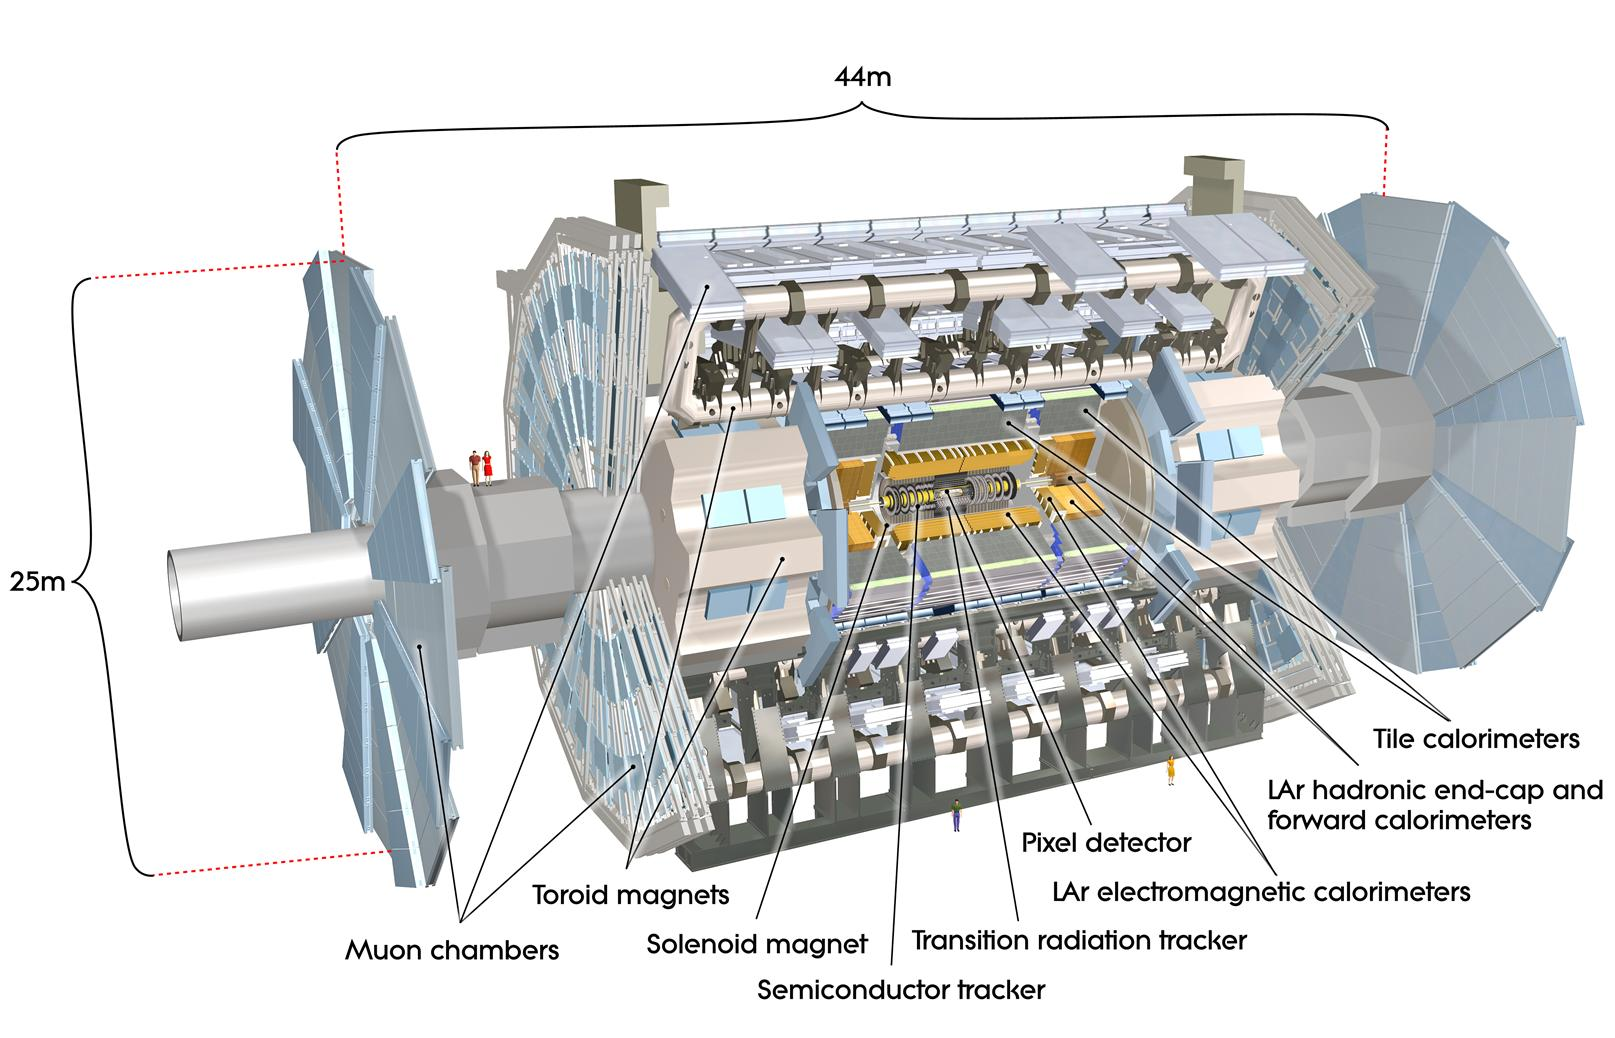
\includegraphics[width=.9\linewidth]{atlas_full}
\end{figure}

\section{Magnets}

\begin{figure}[tbp]
\caption{The ATLAS magnet system. Copyright CERN} \label{fig:atlas_magnets}
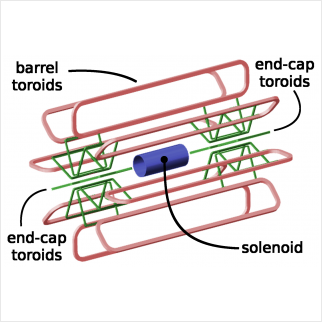
\includegraphics[width=.9\linewidth]{atlas_magnets}
\end{figure}

ATLAS contains multiple magnetic systems.
Primarily, we are concerned with the solenoid, used by the inner detector, and the toroids located outside of the ATLAS calorimeter.
A schematic is shown in \Cref{fig:atlas_magnets}.
These magnetic fields are used to bend charged particles, which subsequently allows one to measure their momentum.

The ATLAS central solenoid is a 2.3 m diameter, 5.3 m long solenoid at the center of the ATLAS detector.
It produces a uniform magnetic field of 2 T.
An important design constraint for the central solenoid was the decision to place it in between the inner detector and the calorimeters.
To avoid excessive energy deposition which could affect calorimeter measurements, the central solenoid must be as transparent as possible\footnotemark.
\footnotetext{This is also one of the biggest functional differences between ATLAS and CMS
In CMS, the solenoid is outside of the calorimeters.}

The toroid system consists of eight air-core superconducting barrel loops, which give ATLAS its distinctive shape.
There are also two endcap air-core magnets.
These produce a magnetic field in a region of approximately 26 m in length and 10 m of radius.
The magnetic field in this region is non-uniform.

\section{Inner Detector}

The ATLAS inner detector consists of three separate tracking detectors, which are known as, in order of increasing distance from the interaction point, the Pixel Detector, Semiconductor Tracker (SCT), and the Transition Radiation Tracker (TRT).
\begin{figure}[tbp]
\caption{The ATLAS inner detector. Copyright CERN} \label{fig:atlas_inner_detector}
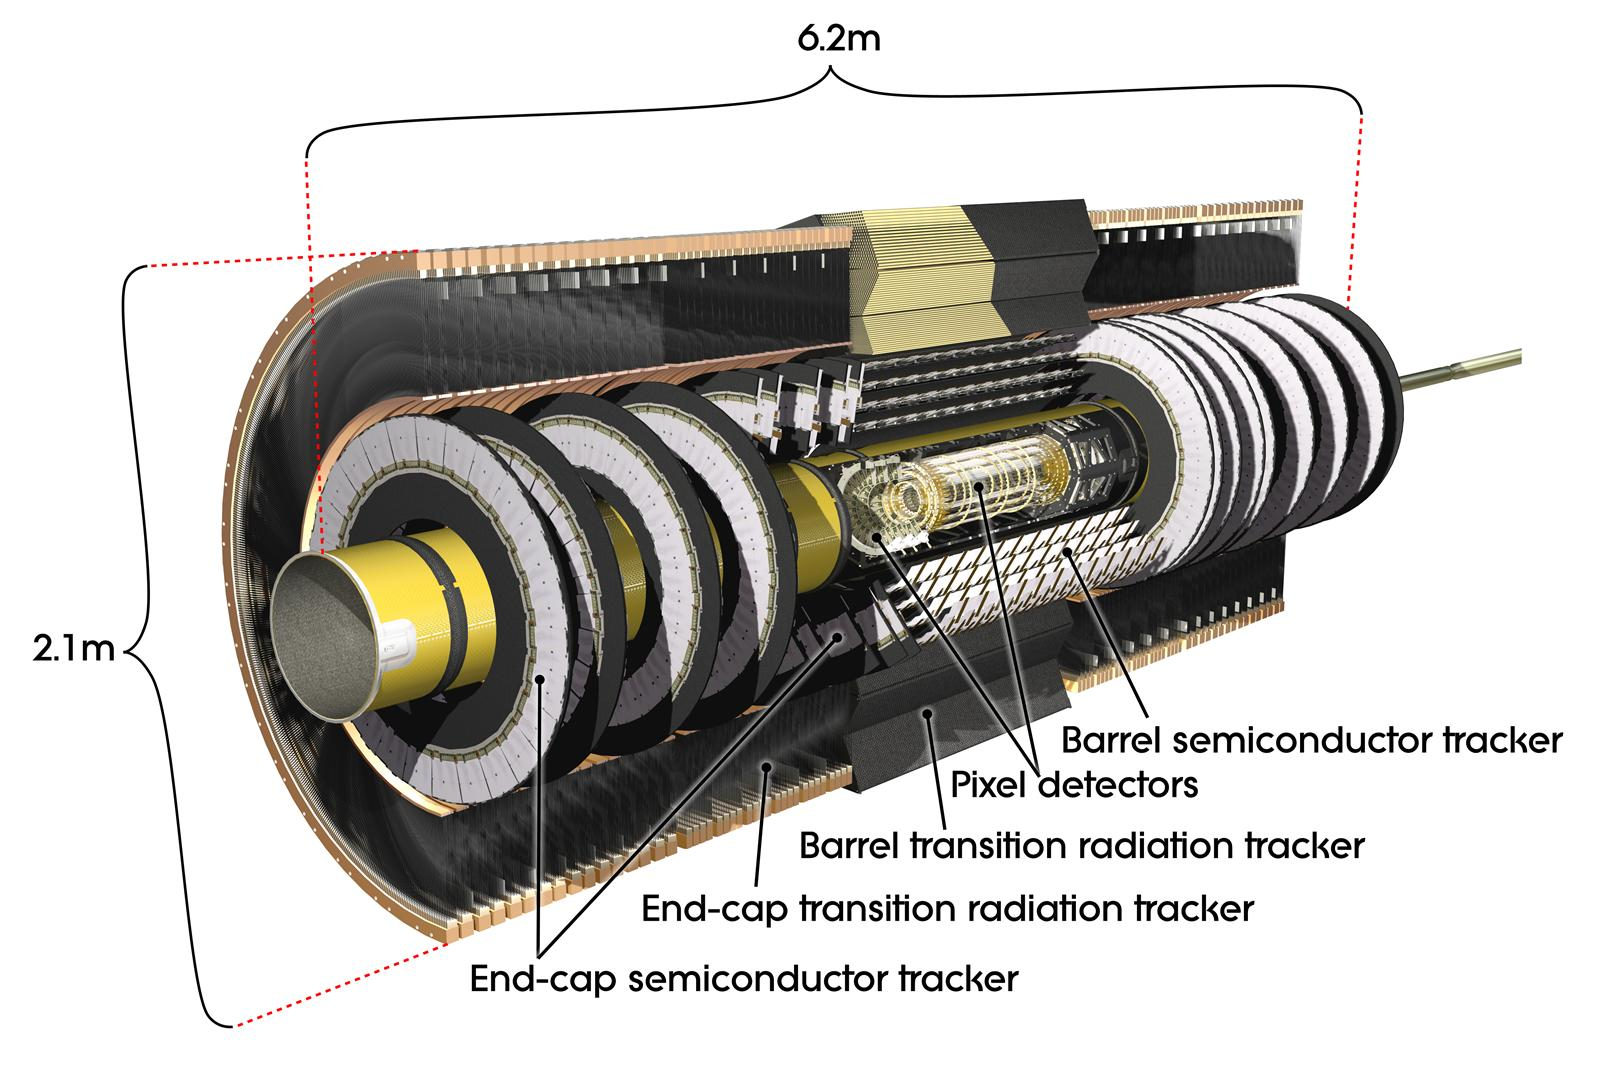
\includegraphics[width=.9\linewidth]{atlas_inner_detector}
\end{figure}
When charged particles pass through these tracking layers, they produce \textit{hits}, which using the known 2 T magnetic field, allows the reconstruction of \textit{tracks}.
Tracks are used as inputs for reconstruction of many higher-level physics objects, such as electrons, muons, photons, and \met.
Accurate track reconstruction is thus crucial for precise measurements of charged particles.

\subsection{Pixel Detector}
\begin{figure}[tbp]
\caption{The ATLAS pixel detector. Copyright CERN} \label{fig:atlas_inner_detector}
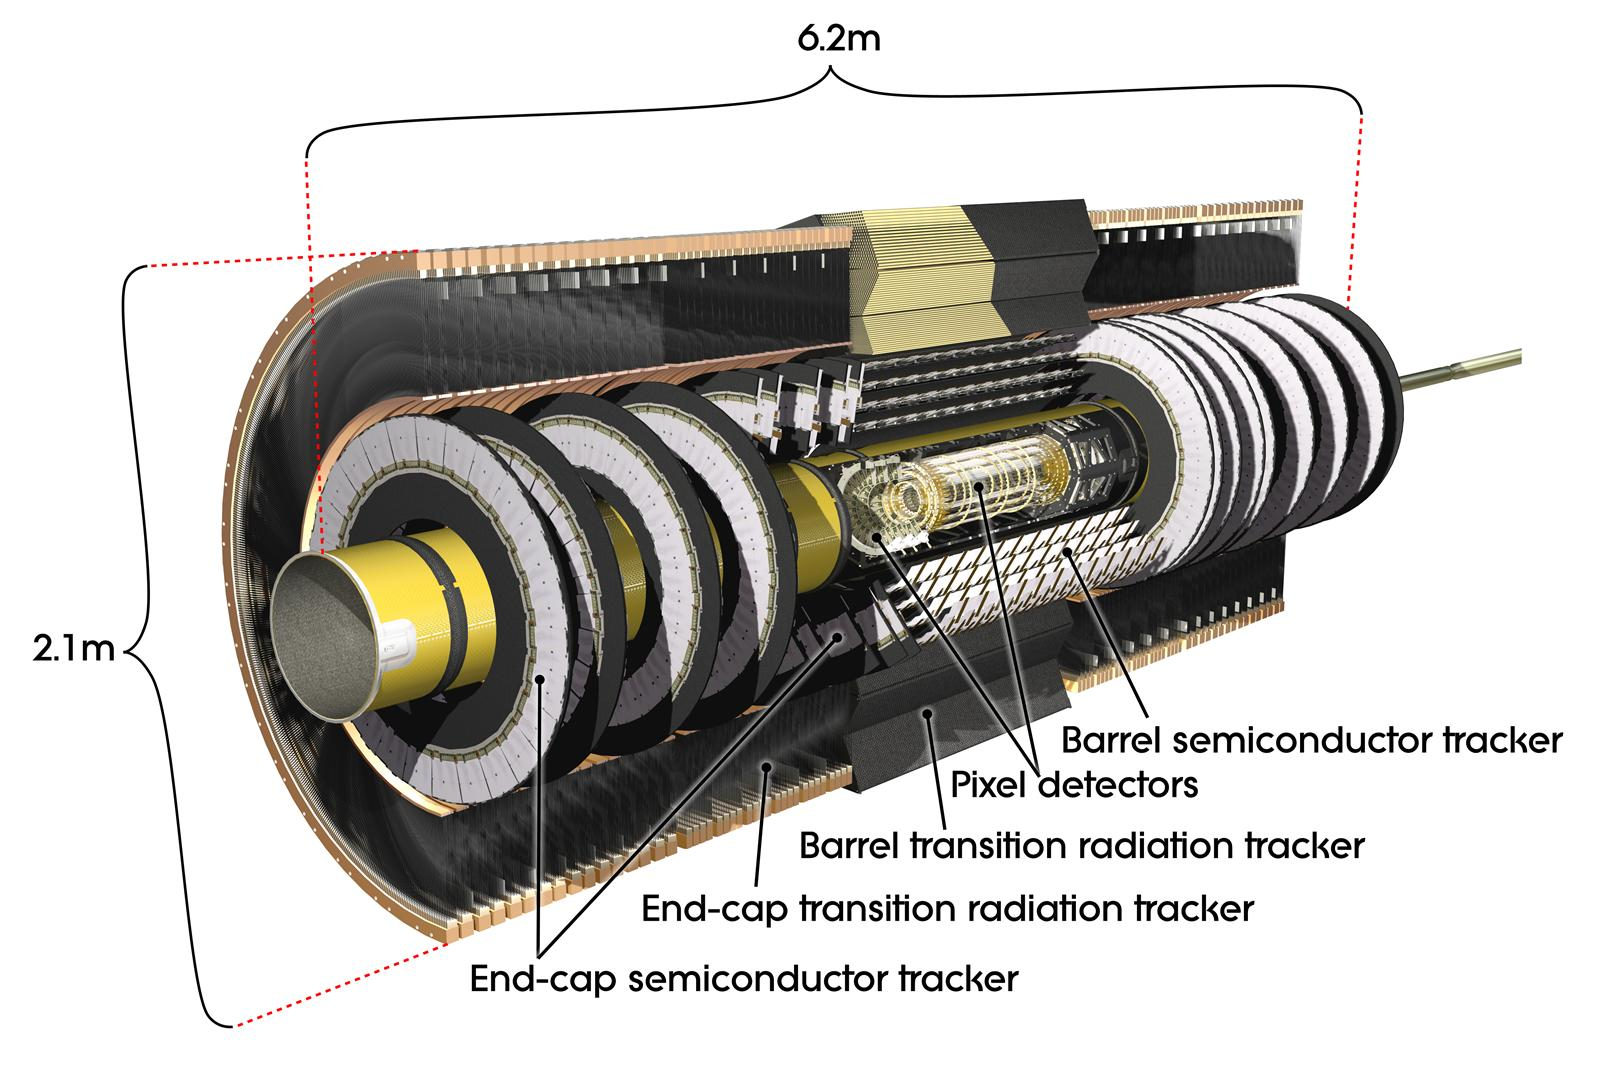
\includegraphics[width=.9\linewidth]{atlas_inner_detector}
\end{figure}

The ATLAS pixel detector consists four layers of silicon ``pixels''~\cite{Aad:2008zz}.
This refers to the segmentation of the active medium into pixels, which provide precise 3D hit locations.
The layers are known as the ``Insertable'' B-Layer (IBL), the B-Layer (or Layer-0), Layer-1, and Layer-2, in order of increasing distance from the interaction point.
These layers are close to the interaction point, and therefore experience significant radiation exposure.

Layer-1, Layer-2, and Layer-3 were installed with the initial construction of ATLAS.
They contain front-end integrated electronics (FEI3s) bump-bonded to 1744 silicon modules.
Each module is 250 $\mu$m in thickness and contains 47232 pixels.
These pixels have planar sizes of 50 x 400 $\mu^2$ or  50 x 600 $\mu^2$, to provide highly accurate location information.
The FEI3s are mounted on long rectangular structures known as staves, which encircle the beam pipe.
A small tilt to each stave allows full coverage in $\phi$.
These layers are at radii of 50.5 mm, 88.5 mm, and 122.5 mm from the interaction point.

The IBL was added to ATLAS after Run1 in 2012 at a radius of 33 mm from the interaction point ~\cite{B-layerRef}.
The IBL was required to preserve the integrity of the pixel detector as radiation damage leads to inoperative pixels in the other layers.
The IBL consists of 448 FEI4 chips, arranged onto 14 staves.
Each FEI4 has 26880 pixels, of planar size 50 x 250 $\mu$m.
This smaller granularity was required due to the smaller distance to the interaction point.

In total, a charged particle passing through the inner detector would expect to leave four hits in the pixel detector.

\subsection{Semiconductor Tracker}
\begin{figure}[tbp]
\caption{A ring of the Semiconductor Tracker. Copyright CERN} \label{fig:sct_photo}
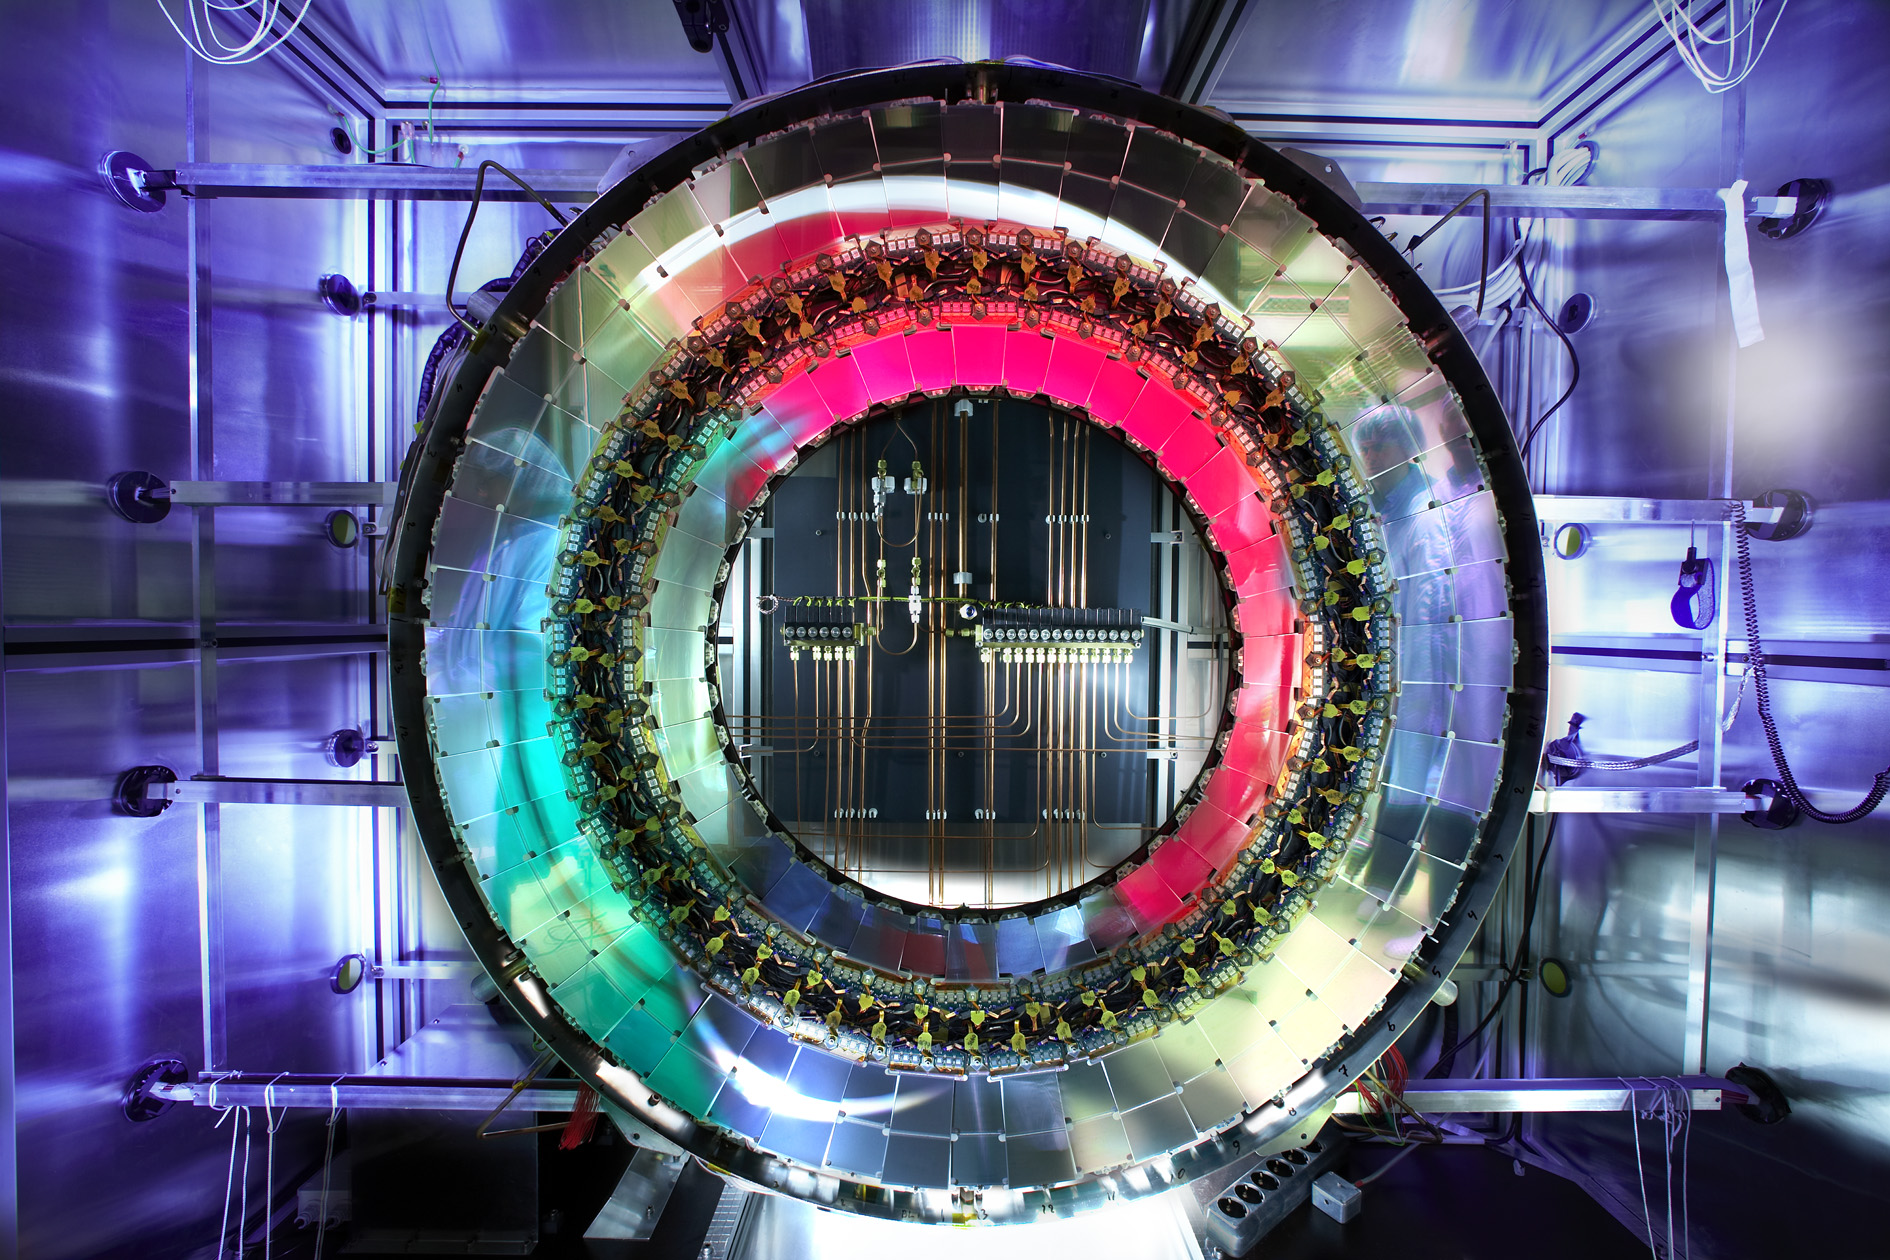
\includegraphics[width=.9\linewidth]{sct_photo}
\end{figure}

The SCT is a silicon strip detector directly beyond Layer-2 of the pixel detector ~\cite{IDET-2013-01}.
The dual-sensors of the SCT contain 2 x 768 individual strips.
Each strip has area 6.4 cm$^2$.
The SCT dual-sensor is double-layered, at a relative angle of 40 mrad.
Together, these layers provide the necessary 3D information for track reconstruction.
There are four of these double-layers, at radii of 284 mm, 355 mm, 427 mm, and 498 mm.
These double-layers provide hits comparable to those of the pixel detector.
The SCT provides an four additional hits to reconstruct tracks for each charged particle.

\subsection{Transition Radiation Tracker}
\begin{figure}[tbp]
\caption{A schematic of the Transition Radiation Tracker. Copyright CERN} \label{fig:trt_schematic}
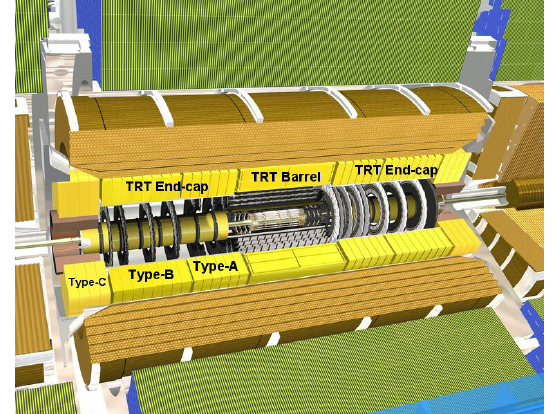
\includegraphics[width=.9\linewidth]{trt_schematic}
\end{figure}
The Transition Radiation Tracker is the next detector radially outward from the SCT.
It contains straw drift tubes.
Each tube contains a tungsten gold-plated wire of 32 $\mu$m diameter held under high voltage (-1530 V) with the edge of the Kapton-aluminum tube.
They are filled with a gas mixture of primarily xenon that is ionized when a charged particle passes through the tube.
The ions are collected by the ``drift'' due to the voltage inside the tubes, which is read out by the electronics.
% This gives so-called ``continuous tracking'' throughout the tube, due to the large number of ions produced.
% The TRT is so-named due to the \textit{transition radiation} (TR) it induces.
Due to the dielectric difference between the gas and tubes, transition radiation is induced.
This is important for distinguishing electrons from their predominant background of minimum ionizing particles.
Generally, electrons have a much larger Lorentz factor than minimum ionizing particles, which leads to additional transition radiation.
This is used to discriminate electrons from background in electron reconstruction.

\section{Calorimetry}
\begin{figure}[tbp]
\caption{The ATLAS calorimeter. Copyright CERN} \label{fig:atlas_calorimeter}
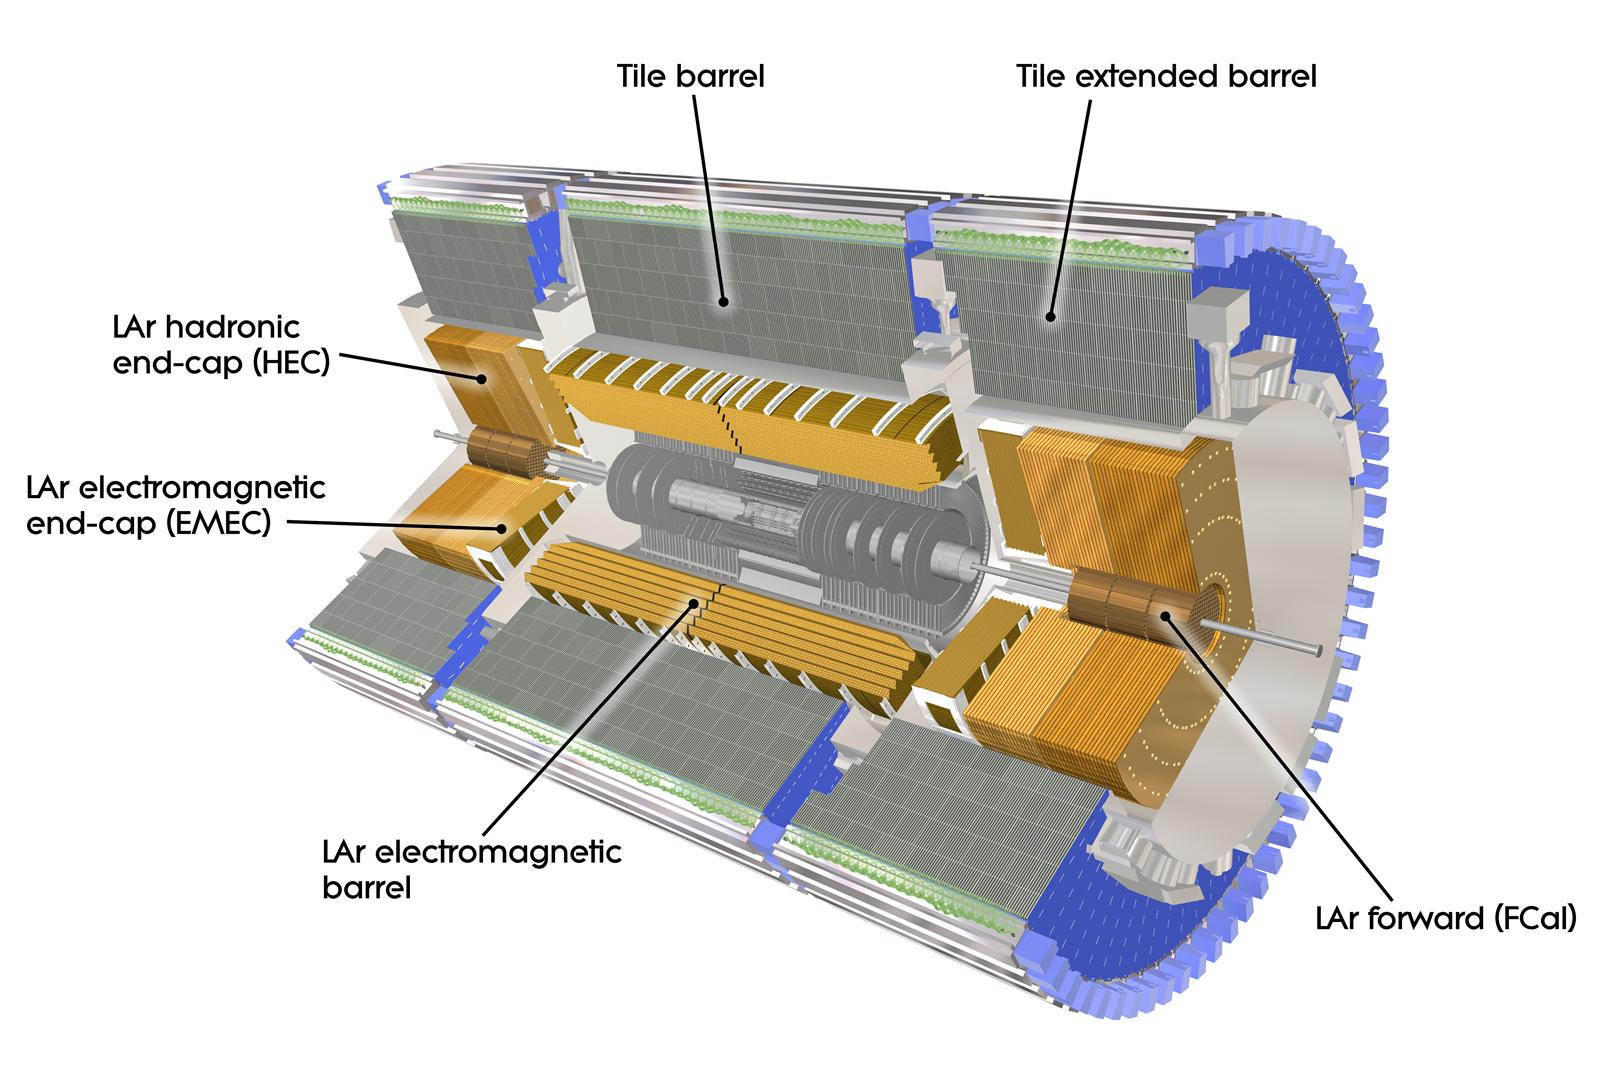
\includegraphics[width=.9\linewidth]{atlas_calorimeter}
\end{figure}

The calorimetry of the ATLAS detector also includes multiple subdetectors which allow precise measurements of the electrons, photons, and hadrons produced in collisions delivered by the LHC.
Calorimeters work by stopping particles in their material and measuring the energy deposition.
This energy is deposited as a cascade of particles induce from interactions with the detector material known as \textit{showers}.
ATLAS uses \textit{sampling} calorimeters, alternating a dense absorbing material to induce showers with an active layer to measure energy depositions by the induced showers.
Since some energy is deposited into the absorption layers as well, the energy depositions must be properly calibrated for the detector.

Electromagnetic objects (electrons and photons) and hadrons have different interaction properties.
We use different types of calorimeters to accurately measure these classes of objects, which we call \textit{electromagnetic} and \textit{hadronic} calorimeters.
ATLAS contains multiple separate calorimeters : the liquid argon (LAr) electromagnetic barrel calorimeter, the Tile barrel hadronic calorimeter, the LAr endcap electromagnetic calorimeter, the LAr endcap hadronic calorimeter, and the LAr Forward Calorimeter (FCal).
Combined, these provide full coverage in $\phi$ up to $|\eta| <4.9$.
They are shown in \Cref{fig:atlas_calorimeter}.

\subsection{Electromagnetic Calorimeters}
\begin{figure}[tbp]
\caption{A schematic of a subsection of the barrel LAr electromagnetic calorimeter. Copyright CERN} \label{fig:lar_schematic}
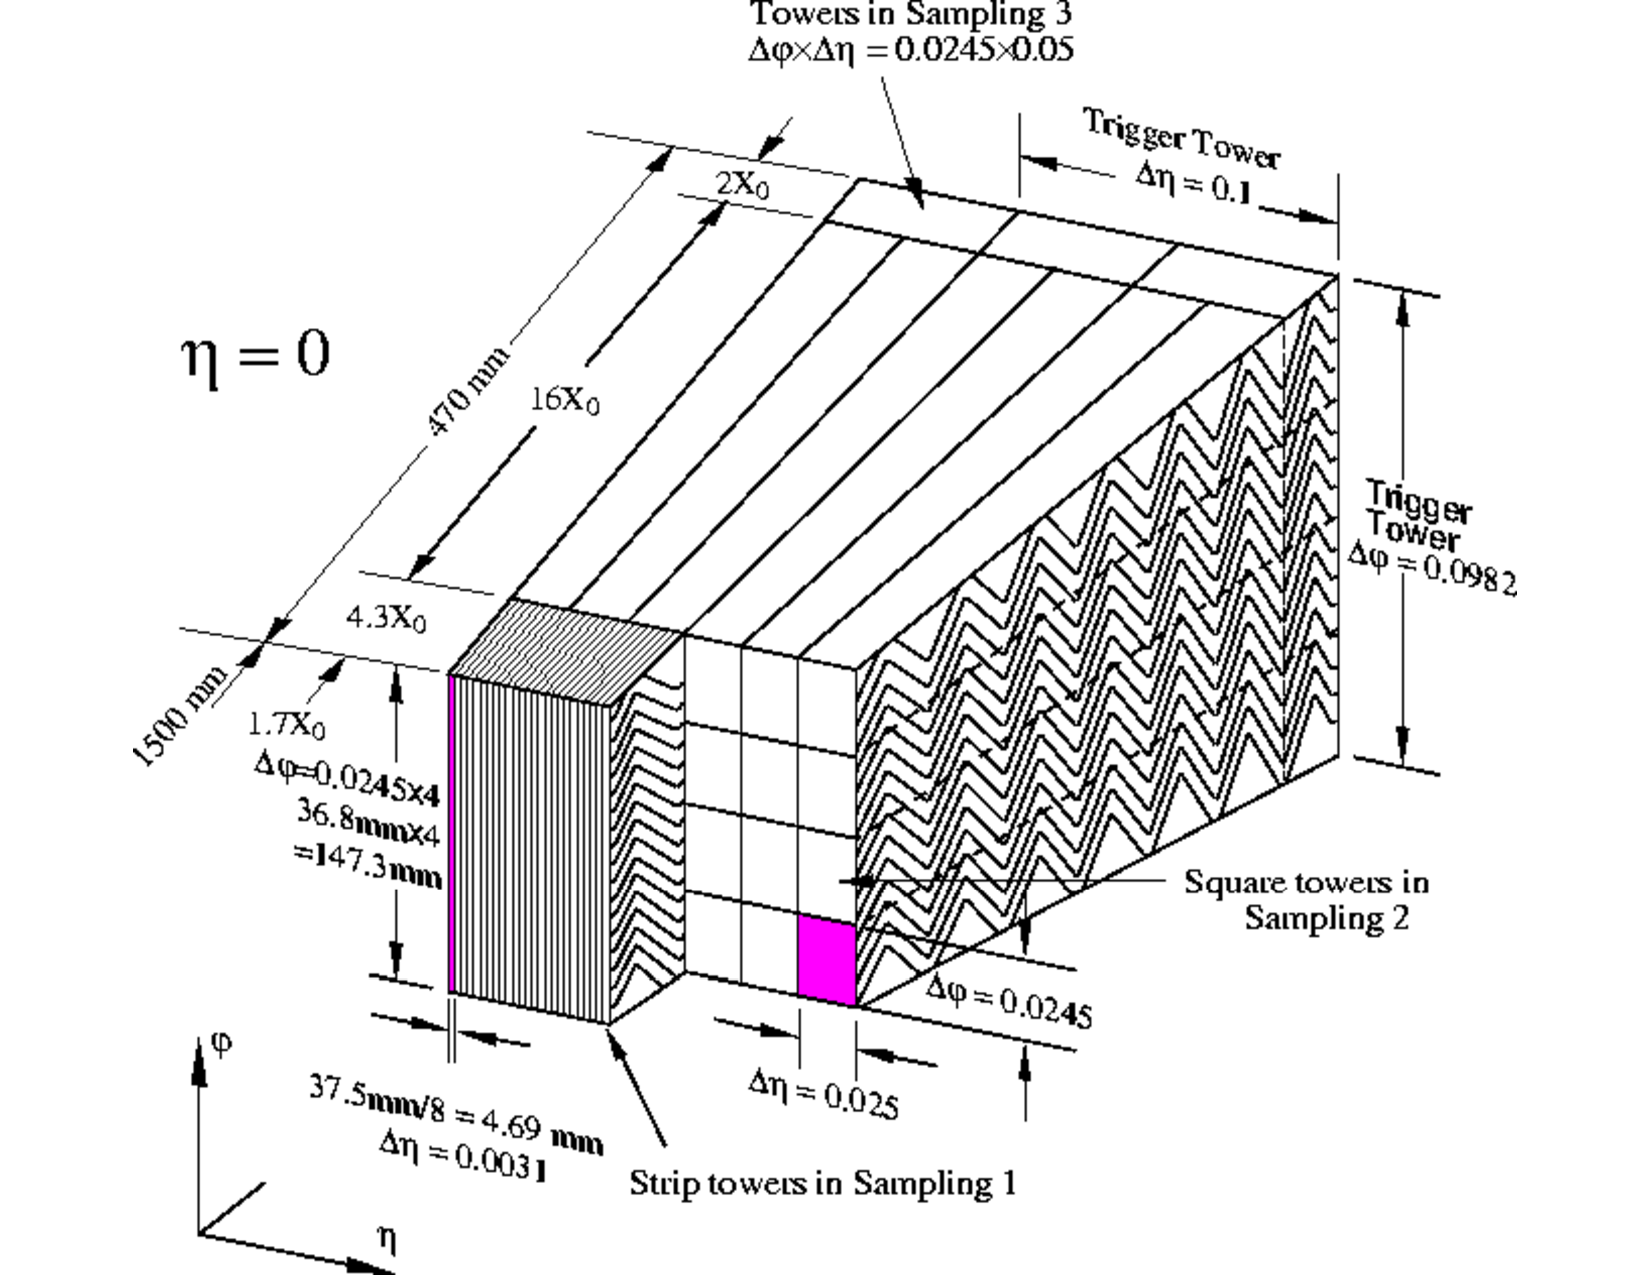
\includegraphics[width=.9\linewidth]{lar_schematic}
\end{figure}

The electromagnetic calorimeters of the ATLAS detector consist of the barrel and endcap LAr calorimeters.
These are arranged into an ``accordion'' shape, shown in \Cref{fig:lar_schematic}, which allows full coverage in $\phi$ and significant coverage in $\eta$ while still allowing support structures for detector operation.
The accordion is made of layers with liquid argon (active detection material) and lead (absorber) to induce electromagnetic showers.
The LAr EM calorimeters are each more than 20 radiation lengths deep, which provides the high stopping power necessary to properly measure the electromagnetic showers.

The barrel component of the LAr EM calorimeter extends from the center of the detector out to $| \eta| <  1.475 $.
The calorimeter has a presampler, which measures the energy of any EM shower induced before the calorimeter.
This has segmentation of $\Delta\eta = 0.025$,$ \Delta\phi = .01$
There are three ``standard'' layers in the barrel, which have decreasing segmentation into calorimeter \textit{cells} as one travels radially outward from the interaction point.
The first layer has segmentation of $\Delta\eta = 0.003, \Delta\phi = .1$, and is quite thin with a depth of 4 radiation lengths.
It provides precise $\eta$ and $\phi$ measurements for incoming EM objects.
The second layer is the deepest at 16 radiation lengths, with a segmentation of $\Delta\eta = 0.025, \Delta\phi = 0.025$.
It is primarily responsible for stopping the incoming EM particles, which dictates its large relative thickness, and measures most of the energy of the incoming particles.
The third layer is only 2 radiation lengths deep, with a rough segmentation of $\Delta\eta = 0.05, \Delta\phi = .025$.
The deposition in this layer is primarily used to distinguish hadrons interacting electromagnetically and entering the hadronic calorimeter from the strictly EM objects which are stopped in the second layer.

The barrel EM calorimeter has a similar overall structure, but extends from $1.4 < |\eta| < 3.2$.
The $\eta$ segmentation is smaller in the endcap than the barrel, while the $\phi$ segmentation is the same.
In total, the EM calorimeters contain about 190000 individual calorimeter cells.


\subsection{Hadronic Calorimeters}
\begin{figure}[tbp]
\caption{A schematic of Tile hadronic calorimeter. Copyright CERN} \label{fig:tile_schematic}
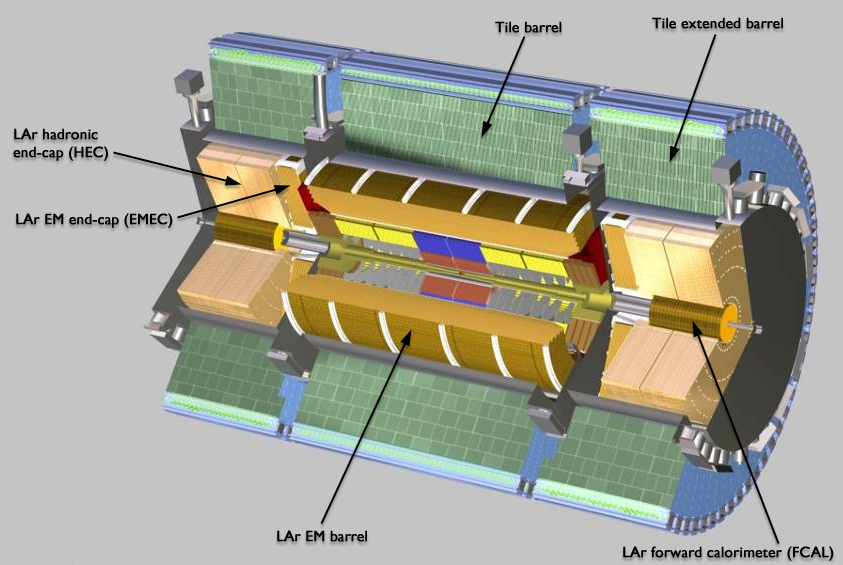
\includegraphics[width=.9\linewidth]{tile_schematic}
\end{figure}

The hadronic calorimetry of ATLAS sits directly outside the EM calorimetry.
It contains three subdetectors : the barrel Tile calorimeter, the endcap LAr calorimeter, and the Forward  LAr Calorimeter.
Similar to the EM calorimeters, these are sampling calorimeters that alternate steel (dense material) with an active layer (plastic scintillator).

The barrel Tile calorimeter extends out to $|\eta| < 1.7$.
It has three layers, which combined give about 10 interactions lengths to provide excellent stopping power for hadrons.
This is critical to avoid excess \textit{punchthrough} to the muon spectrometer beyond the hadronic calorimeters.
The first layer has a depth of 1.5 interaction lengths.
The second layer is again the thickest at a depth of 4.1 interaction lengths.
Most of the energy of incoming particles is deposited in the second layer.
Both the first and second layer have segmentation of $\Delta\eta = 0.1, \Delta\phi = 0.1$.
Generally, one does not need as fine granularity in the hadronic calorimeter, since the energy depositions in the hadronic calorimeters will be summed into the composite objects as jets.
The third layer has a thickness of 1.8 interaction lengths, with a segmentation of $\Delta\eta = 0.2, \Delta\phi = 0.1$.
The use of multiple layers gives information about the induces hadronic shower as it propagates through the detector material.

The endcap LAr hadronic calorimeter is a sampling calorimeter which covers the region $1.5 < |\eta| < 3.2$.
Liquid argon is the the active material and it uses a copper absorber.
Unlike the other sampling calorimeters in ATLAS, it does not use the accordion shape.
Instead, it is a flat detector perpendicular to the interaction point.
The segmentation varies with $\eta$, ranging from cells of size $\Delta\eta = 0.1, \Delta\phi = 0.1$ in the center region to $\Delta\eta = 0.2, \Delta\phi = 0.2$ in the forward region.

The forward LAr calorimeter is the last subdetector of the ATLAS calorimetry.
Of those subdetectors which are used for standard reconstruction techniques, the FCal sits at the most extreme values of $ 3.1 < |\eta| < 4.9$.
The FCal itself is made of three subdetectors: the electromagnetic FCal1 and hadronic FCal2 and FCal3.
The absorber in FCal1 is copper, with a liquid argon active medium.
FCal2 and FCal3 also use a liquid argon active medium, with a tungsten absorber.

\section{Muon Spectrometer}
\begin{figure}[tbp]
\caption{The ATLAS muon spectrometer. Copyright CERN} \label{fig:atlas_muon_spectrometer}
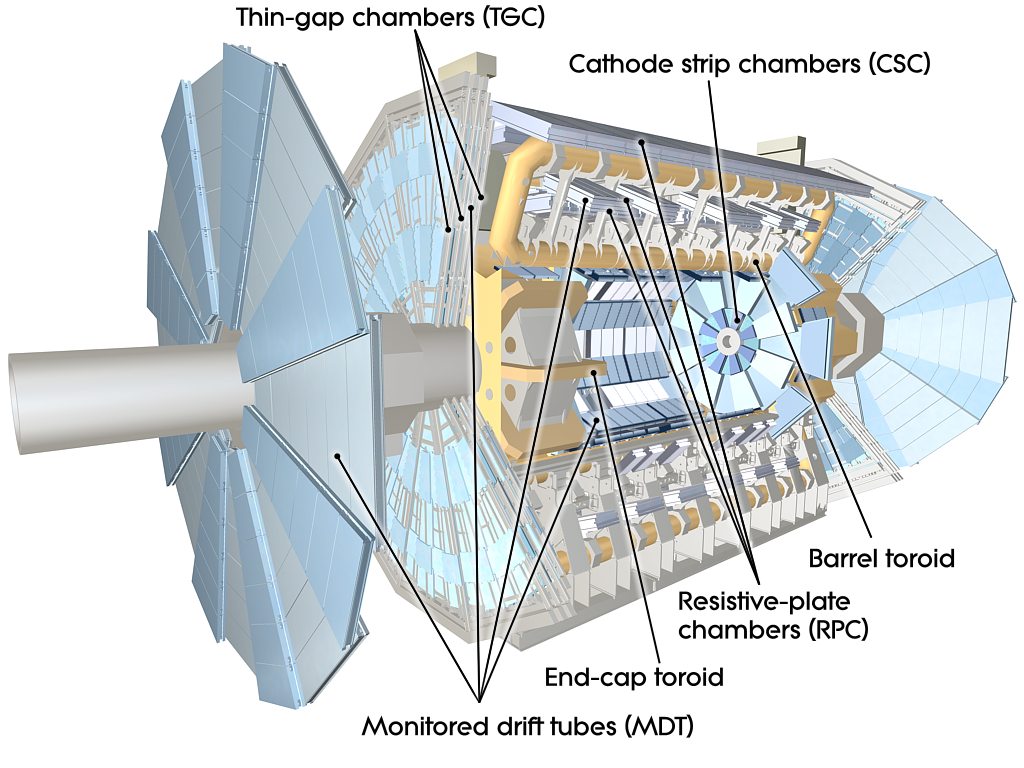
\includegraphics[width=.9\linewidth]{atlas_muon_spectrometer}
\end{figure}

\begin{figure}[tbp]
\caption{A schematic in $z/\eta$ showing the location of the subdetectors of the muon spectrometer. Copyright CERN} \label{fig:atlas_schematic_muon_spectrometer}
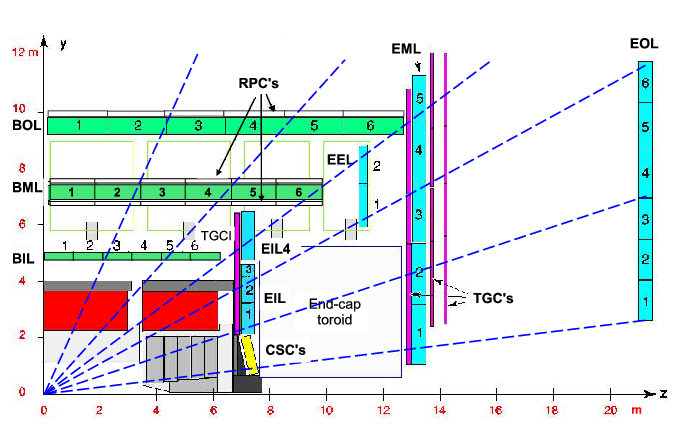
\includegraphics[width=.9\linewidth]{atlas_schematic_muon_spectrometer}
\end{figure}

The muon spectrometer sits outside the hadronic calorimetry, with pseudorapidity coverage out to $|\eta| < 2.7$.
The MS is a huge detector, with some detector elements existing as far as 11 m in radius from the interaction point.
This system is used almost exclusively to measure the momenta of muons.
These systems provide a rough measurement, which is used in triggering (described in \Cref{sec:trigger}), and a precise measurement to be used in offline event reconstruction.
The MS produces tracks in a similar way to the ID.
The hits in each subdetector are recorded and then tracks are produced from these hits.
Muon spectrometer tracks are largely independent of the ID tracks due to the independent solenoidal and toriodal magnet systems used in the ID and MS respectively.
The MS consists of four separate subdetectors: the barrel region is covered by the Resistive Plate Chambers (RPCs) and Monitored Drift Tubes (MDTs) while the endcaps are covered by MDTs, Thin Gap Chambers (TGCs), and Cathode Strip Chambers (CSCs).

\subsection{Monitored Drift Tubes}
\begin{figure}[tbp]
\caption{Schematic of a Muon Drift Tube chamber. Copyright CERN} \label{fig:mdt_chamber}
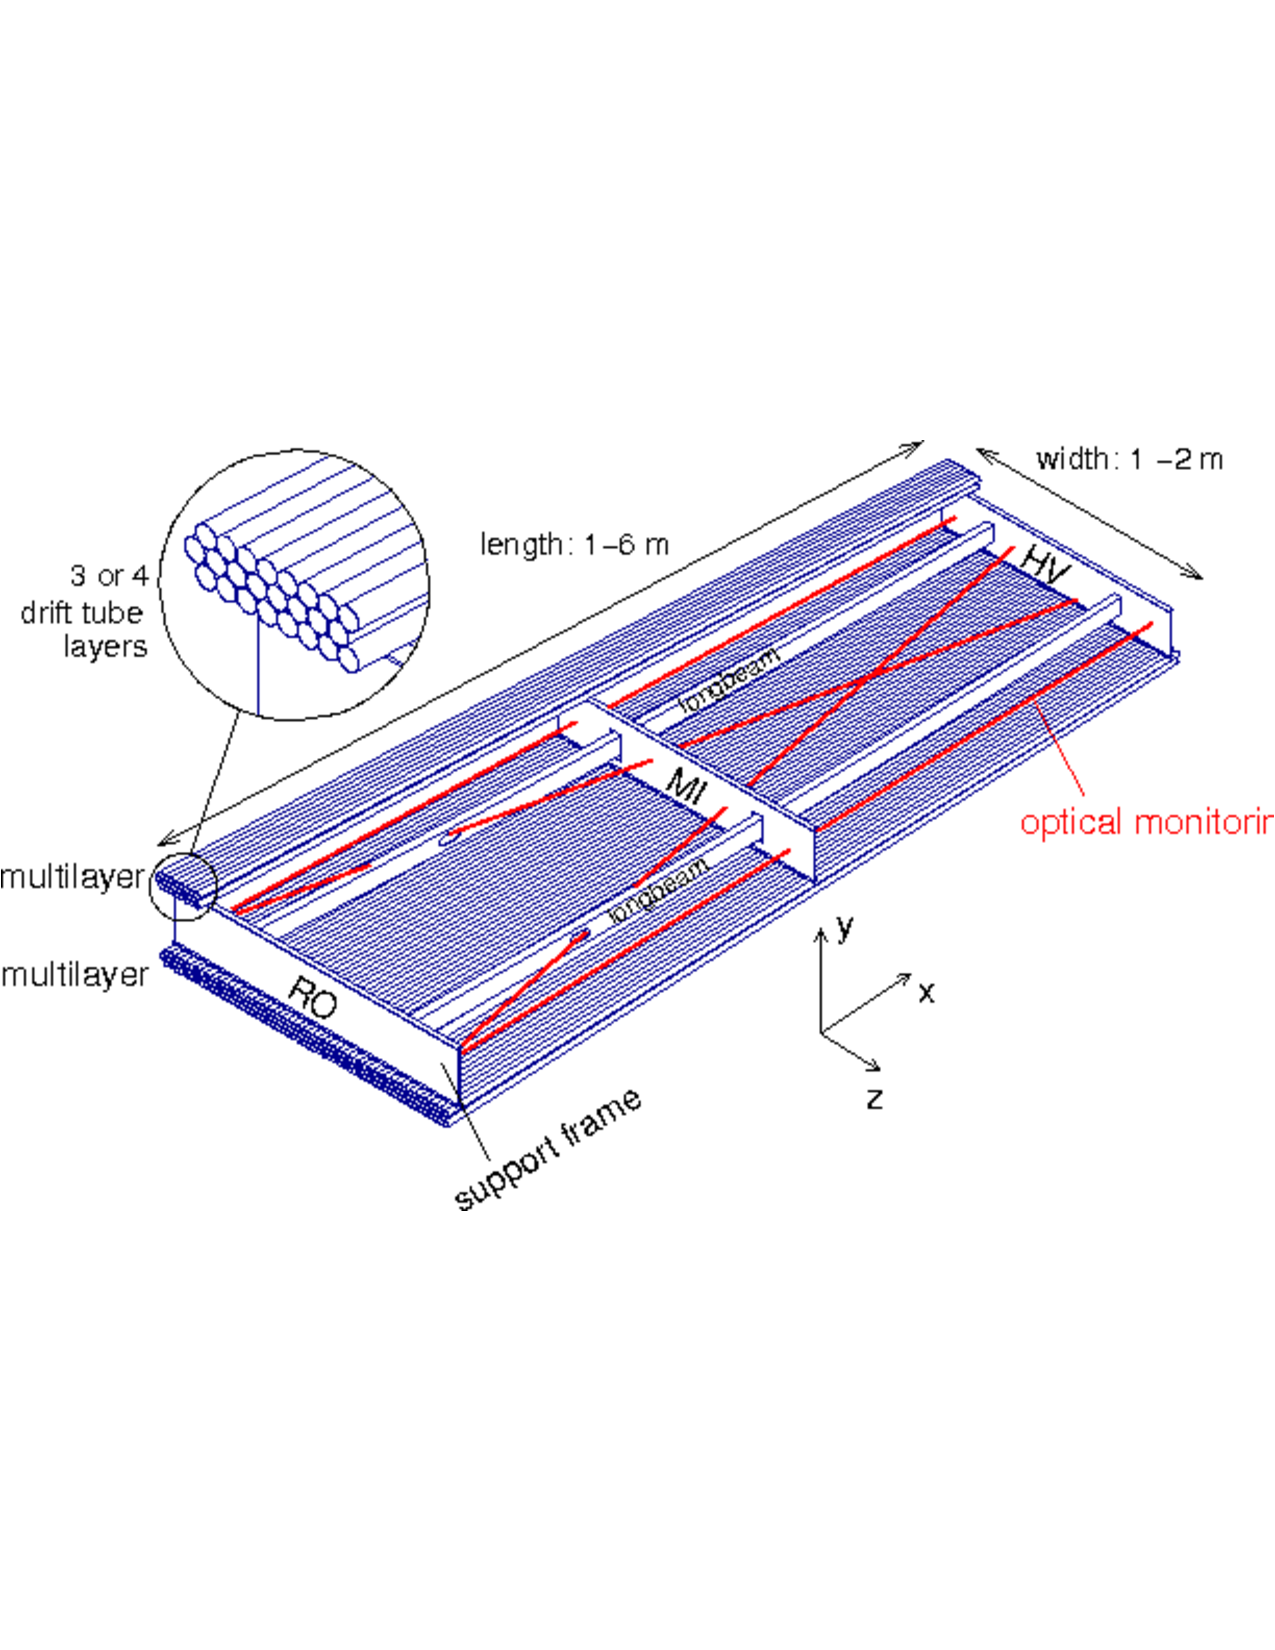
\includegraphics[width=.9\linewidth]{mdt_chamber}
\end{figure}

The MDT system is the largest individual subdetector of the MS.
MDTs provide precision measurements of muon momenta as well as fast measurements used for triggering.
There are 1088 MDT chambers providing coverage out to pseudorapidity $|\eta| < 2.7 $.
Each consists of an aluminum tube containing an argon-CO$_2$ gas mixture.
In the center of each tube there 50 $\mu$m diameter tungsten-rhenium wire at a voltage of 3080 V.
A muon entering the tube will induce ionization in the gas, which will ``drift'' towards the wire due to the voltage.
One measures this ionization as a current in the wire.
The current comes with a time measurement related to how long it takes the ionization to drift to the wire.

These tubes are layered in a pattern shown in \Cref{fig:mdt_chamber}.
Combining the measurements from the tubes in each layer gives good position resolution.
The system consists of three subsystems of these layers, at 5 m, 7 m, and 9 m from the interaction point.
The innermost layer is directly outside the hadronic calorimeter.
The combination of these three measurements gives precise momenta measurements for muons.

\subsection{Resistive Plate Chambers}

The RPC system is alternated with the MDT system in the barrel
The first two layers of RPC detectors surround the second MDT layer while the third is outside the final MDT layer.
The RPC system covers pseudorapidity $|\eta| < 1.05 $.
Each RPC consists of two parallel plates at a distance of 2 mm surrounding a C$_2$H$_2$F$_4$ mixture.
The electric field between these plates is 4.9k kV/mm.
Just as in the MDTs, an incoming muon ionizes the gas, and the deposited ionization is collected by the detector (in this case on the plates).
It is quite fast, but with a relatively poor spatial resolution of 1 cm.
Still, it can provide reasonable $\phi$ resolution due to its large distance from the interaction point.
This is most useful in triggering, where the timing requirements are quite severe.
The RPCs also complement the MDTs by providing a measurement of the non-bending coordinate.

\subsection{Cathode Strip Chambers}
\begin{figure}[tbp]
\caption{Photo of the installation of Cathode Strip Chambers and Monitored Drift Tubes. Copyright CERN} \label{fig:csc_photo}
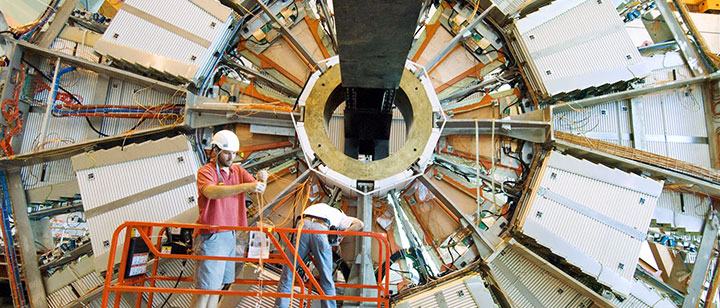
\includegraphics[width=.9\linewidth]{csc_photo}
\end{figure}

The CSCs are used in place of MDTs in the first layer of the endcaps.
This region, at $2.0 < |\eta| < 2.7$, has higher particle multiplicity at close distance to the interaction point from low-energy photons and neutrons.
The MDTs are not equip to deal with the high particle rate in this region, so the CSCs were designed to deal with this deficiency.

Each CSC consists multiwire proportional chambers, oriented radially outward from the interaction point.
These chambers overlap partially in $\phi$.
The wires contain a gas mixture of argon and CO$_2$, which is ionized when muons enter.
The detectors operate with a voltage of 1900 V, with much lower drift times than the MDTs.
They provide less hits than MDTs, but their lower drift times lower uptime and reduce the amount of detector overload.

The CSCs are arranged into four planes on the wheels of the muon spectrometer, as seen in Fig.\Cref{fig:csc_photo}.
There are 32 CSCs in total, with 16 on each side of the detector in $\eta.$

\subsection{Thin Gap Chambers}
\begin{figure}[tbp]
\caption{Photo of a muon Big Wheel, consisting of Thin Gap Chambers. Copyright CERN} \label{fig:tgc_photo}
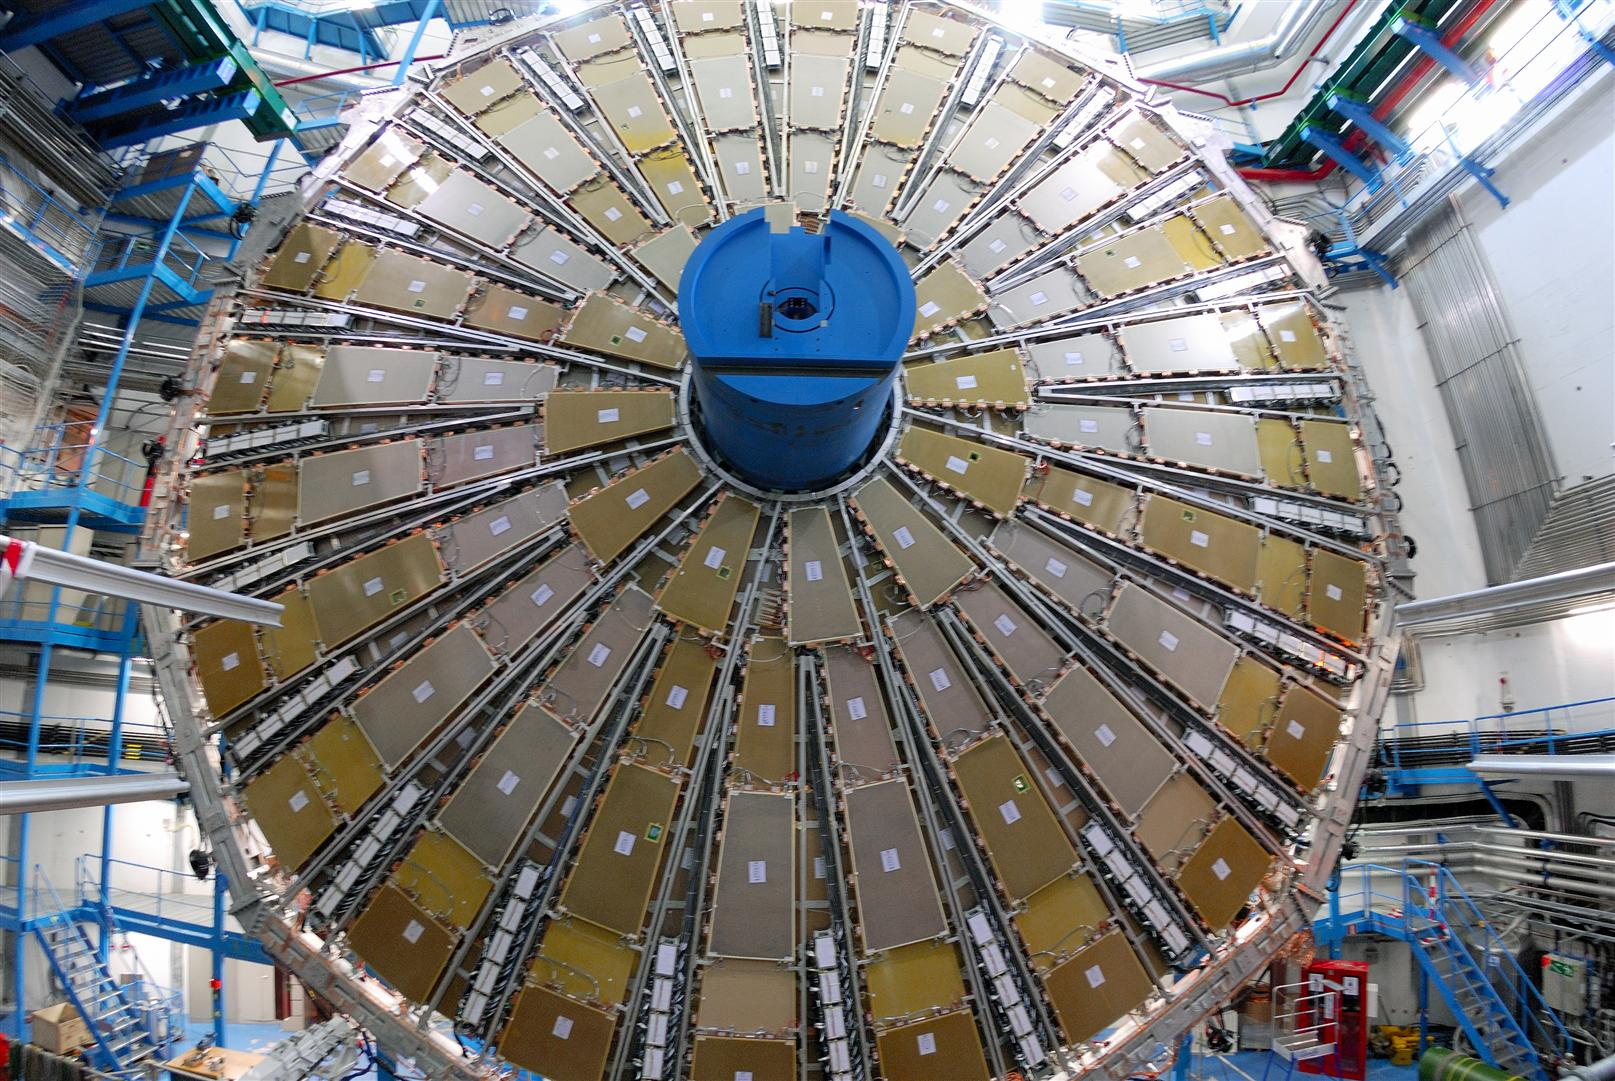
\includegraphics[width=.9\linewidth]{tgc_photo}
\end{figure}

The TGCs serve the purpose of the RPCs in the endcap at pseudorapidity of $1.05 < |\eta| < 2.4 $, by providing fast measurements used for triggering.
They are multiwire proportional chambers similar to the CSCs.
The fast readouts necessary for triggering are provided by a high electric field and a small wire-to-wire distance of 1.8 mm.
These detectors provide both $\eta$ and $\phi$ information, allowing the trigger to use as much information as possible when selecting events.

\section{Trigger System}\label{sec:trigger}

The data rate delivered by the LHC is staggering ~\cite{ATL-DAQ-PUB-2016-001}.
In the 2016 dataset, the collision rate was 40 MHz, meaning a \textit{bunch spacing} of 25 ns.
In each of the event, there are many proton-proton collisions.
Most of the collisions are uninteresting, such as elastic scattering of protons, or even inelastic scattering leading to low-energy dijet events.
These low-energy events have have been studied in detail in previous experiments.

Even if one is genuinely interested in these events, it's \textit{impossible} to save all of the information available in each event.
If all events were written ``to tape'' (as the jargon goes), ATLAS would store terabytes of data per second.
We are limited to only about 1000 Hz readout by computing processing time and storage space.
We thus implement a \textit{trigger} which provides fast inspection of events to drastically reduce the data rate from the 40 MHz provided by the LHC to the 1000 Hz we can write to tape for further analysis.

The ATLAS trigger system consists of a two-level trigger, known as the Level-1 trigger (L1 trigger) and the High-Level Trigger (HLT)\footnotemark.
\footnotetext{In Run1, ATLAS ran with a three-level trigger system.
The L1 was essentially as today.
The HLT consisted of two separate systems known as the L2 trigger and the Event Filter (EF).
This was changed to the simpler system used today during the shutdown between Run1 and Run2.
}
Trigger selections are organized into \textit{trigger chains}, where events passing a particular L1 trigger are passed to a corresponding HLT trigger.
For example, one would require a particular high-\pt muon at L1, with additional quality requirements at HLT.
One can also use HLT triggers as prerequisites for each other, as is done in some triggers requiring both jets and \met.

\subsection{Level-1 Trigger}

The L1 trigger is hardware-based, and provides the very fast rejection needed to quickly select events of interest.
The L1 trigger uses only what is known as \textit{prompt} data to quickly identify interesting events.
Only the calorimeters and the triggering detectors (RPCs and TGCs)  of the MS are fast enough to be considered at L1, since the tracking reconstruction algorithms used by the ID and the more precise MS detectors are very slow.
This allows quick identification of events with the most interesting physical objects: large missing transverse momentum and high-\pt electrons, muons, and jets.

L1 trigger processing is done locally.
This means that events are selected without considering the entire available event.
Energy deposits over some threshold are reconstructed as \textit{regions of interest} (RoIs).
These RoIs are then compared using pattern recognition hardware to ``expected'' patterns for the given RoIs.
Events with RoIs matching these expected patterns are then handed to the HLT through the Central Trigger Processor.
This step lowers the data rate down to about 75 kHz.

\subsection{High-Level Trigger}

After passing the L1 trigger, events are passed to the HLT, which takes the incoming data rate from \order 75 kHz down to the \order 1 kHz that can be written to tape.
The HLT performs much like a simplified offline reconstruction, using many common quality and analysis cuts to eliminate uninteresting events.
This is done by using computing farms located close to the detector, which process events in parallel.
Individually, each event which enters the computing farms takes about 4 seconds to reconstruct.
However, some events take significantly longer to reconstruct, which necessitates careful monitoring of the HLT to ensure smooth operation.

HLT triggers are targeted to a particular physics process, such as a \met trigger, single muon trigger, or multijet trigger.
The collection of all triggers is known as the trigger \textit{menu}.
Since many low-energy particles are produced in collisions, it is necessary to set a \textit{trigger threshold} on the object of interest.
Due to the changing luminosity conditions of the LHC, these thresholds change constantly.
The most common strategy is to increase the trigger thresholds with increasing instantaneous luminosity.
This allows an approximately constant number of events to be written for further analysis.
Triggers which have rates higher than those designated by the menu are \textit{prescaled}.
A prescaled trigger only records every $n$th event which passes the trigger requirements, where $n$ is the prescale value.
One wishes to investigate all data events passing some set of analysis cuts, so often one uses the ``lowest threshold unprescaled trigger''.
\textit{Turn-on curves} allow one to select the needed offline analysis cut to ensure the trigger is fully efficient.
An example turn-on curve for the \met triggers used in the signal region of this analysis is shown in \Cref{fig:met_turnon}.
\begin{figure}[tbp]
\caption{Turn-on curves for a variety of \met triggers} \label{fig:met_turnon}
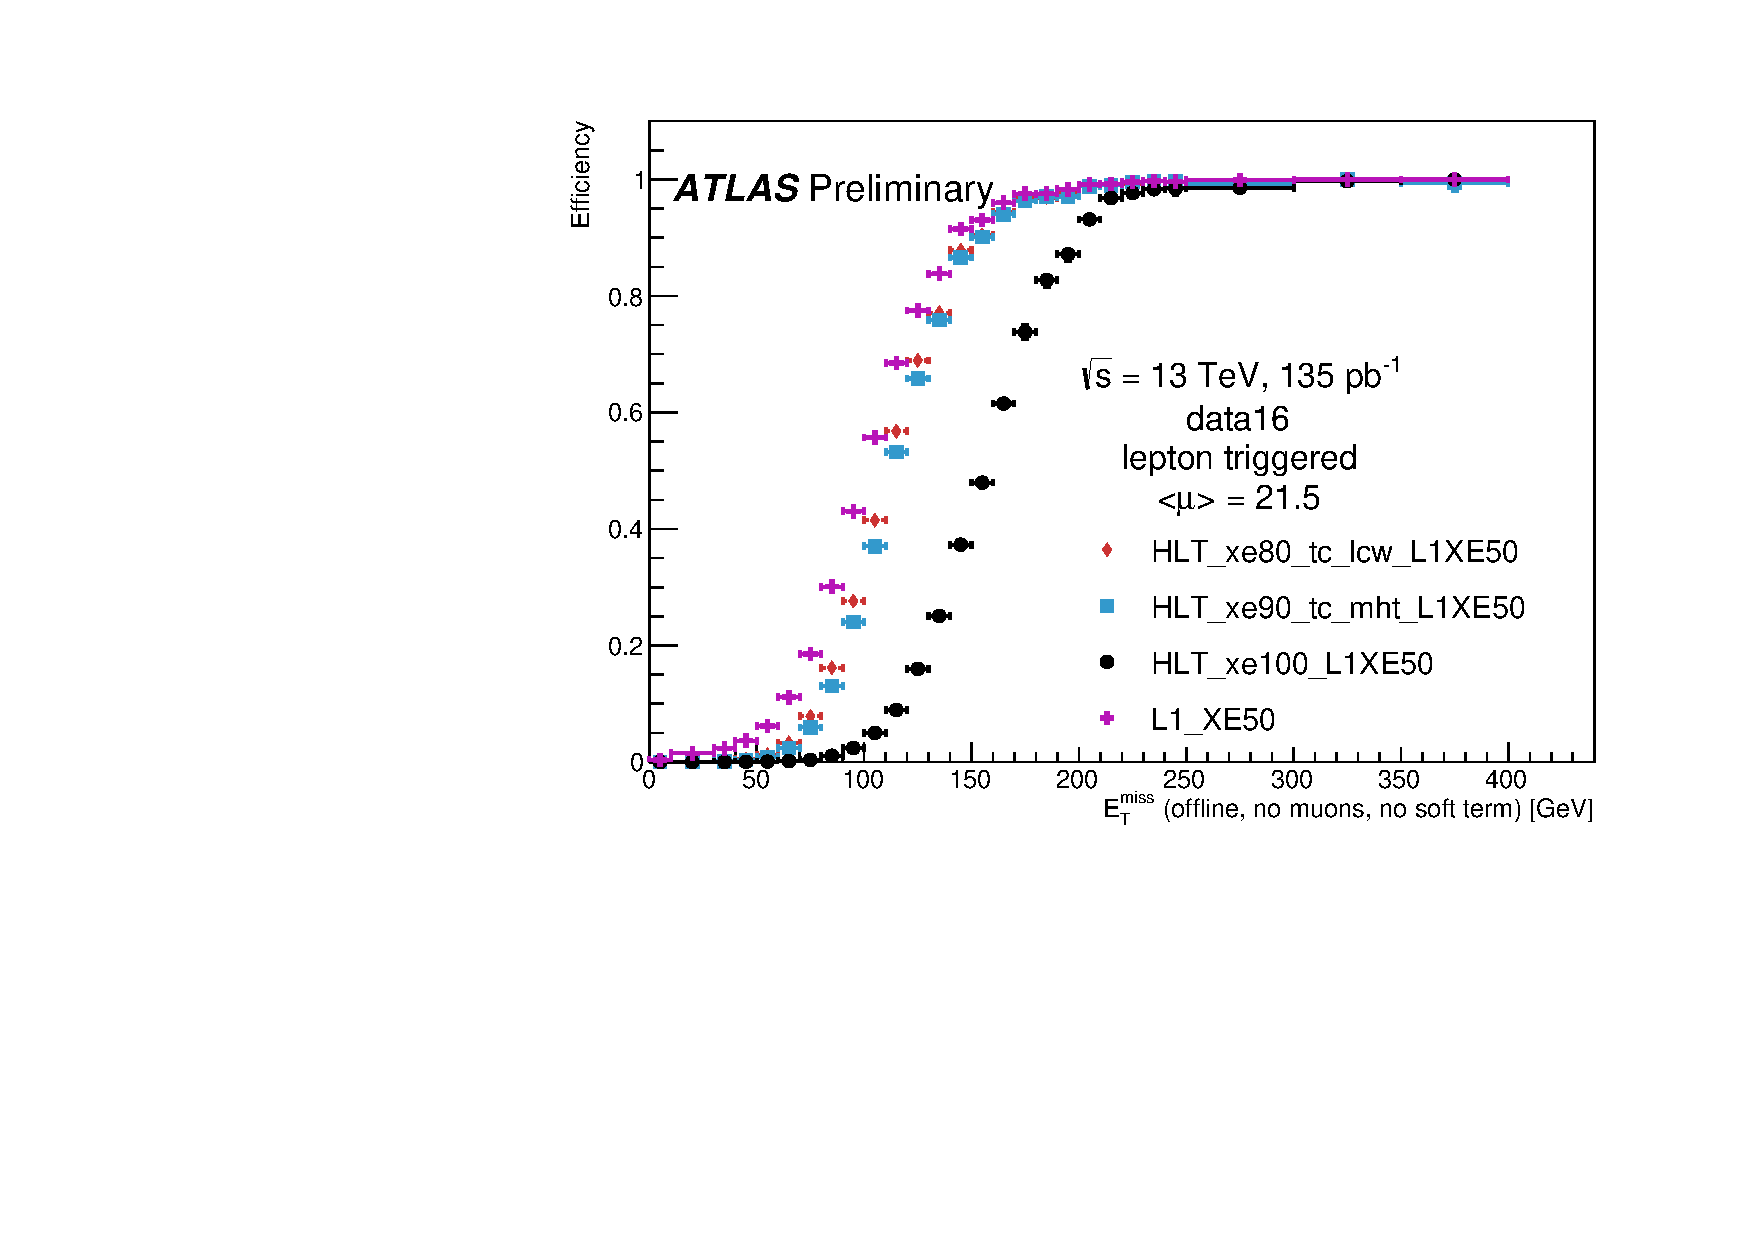
\includegraphics[width=.9\linewidth]{2016-05-16-UpdatedTurnOns}
\end{figure}

The full set of the lowest threshold unprescaled triggers considered here can be found in \Cref{tab:triggers}.
These are the lowest unprescaled triggers associated to the SUSY signal models and Standard Model backgrounds considered in this thesis.
More information can be found in ~\cite{ATL-DAQ-PUB-2016-001}.

% SR events are required to pass HLT_xe70 trigger,
% • CRW, CRT, CRZ events are required to pass HLT_mu24_iloose_L1MU15 || HLT_mu50 for muons
% and HLT_e24_lmedium_iloose_L1EM20VH (HLT_e24_lhmedium_iloose_L1MU18VH for MC)
% || HLT_e60_lhmedium || HLT_e120_lhloose for electrons,
% • CRY events are required to pass HLT_g120_loose trigger.
% The following triggers are used in this analysis for 2016:
% • SR events are required to pass HLT_xe100_mht_L1XE50 trigger,
% • CRW, CRT, CRZ events are required to pass HLT_mu24_ivarmedium || HLT_mu50 for muons and
% HLT_e24_lhtight_nod0_ivarloose || HLT_e60_lhmedium_nod0 || HLT_e140_lhloose_nod0 for
% electrons,
% • CRY events are required to pass HLT_g140_loose trigger.
\begin{sidewaystable}[htbp]
\caption{High-Level Triggers used in this thesis.
Descriptions of loose, medium, tight, and isolated can be found in ~\cite{ATL-DAQ-PUB-2016-001}.
The d$_0$ cut refers to a quality cut on the vertex position, which was removed from many triggers in 2016 to increase sensitivity to displaced vertex signals.
For most triggers, the increased thresholds in 2015 compared to 2016 were designed to keep the rate approximately equal.
}\label{tab:triggers}
\centering
\begin{tabularx}{\textwidth}{| l | l | l | l | l | l | l|}
\hline
Physics Object & Trigger                                   & \pt Threshold (GeV) & Level-1 Seed         & Requirements      & Rate (Hz) \\
\hhline{|=|=|=|=|=|=}
\multicolumn{6}{|l|}{\textbf{2015 Data}} \\
\met           & \hlttrig{xe70}                            & 70                  & \trigtt{L1\_XE50}    & -                            & 60                    \\
Muon           & \hlttrig{mu24\_iloose}            & 24                  & \trigtt{L1\_MU15}    & isolated, loose              & 130                   \\
Muon           & \hlttrig{mu50}                            & 50                  & \trigtt{L1\_MU15}    & -                            & 30                    \\
Electron       & \hlttrig{e24\_lhmedium\_iloose} & 24                  & \trigtt{L1\_EM20VH}  & medium OR isolated, loose    & 140                   \\
Electron       & \hlttrig{e60\_lhmedium}                   & 60                  & \trigtt{L1\_EM20VH}  & medium                       & 10                    \\
Electron       & \hlttrig{e120\_lhloose}                   & 120                 & \trigtt{L1\_EM20VH}  & loose                        & $<$10                   \\
Photon         & \hlttrig{g120\_loose}                     & 120                 & \trigtt{L1\_EM20VH}  & loose                        & 20                    \\
\hhline{|=|=|=|=|=|=}
\multicolumn{6}{|l|}{\textbf{2016 Data}} \\
\met           & \hlttrig{xe100\_mht\_L1XE50}              & 100                 & \trigtt{L1\_XE50}    & -                            & 180                   \\
Muon           & \hlttrig{mu24\_ivarmedium}                & 24                  & \trigtt{L1\_MU20}    & medium                       & 120                   \\
Muon           & \hlttrig{mu50}                            & 50                  & \trigtt{L1\_MU20}    & -                            & 40                    \\
Electron       & \hlttrig{e24\_lhtight\_nod0}   & 24                  & \trigtt{L1\_EM22VHI} & tight with no d$_0$ OR loose & 110                   \\
Electron       & \hlttrig{e60\_lhmedium\_nod0}             & 60                  & \trigtt{L1\_EM22VHI} & medium with no d$_0$         & 10                    \\
Electron       & \hlttrig{e140\_lhloose\_nod0}             & 140                 & \trigtt{L1\_EM22VHI} & loose with no d$_0$          & $<$10                   \\
Photon         & \hlttrig{g140\_loose}                     & 140                 & \trigtt{L1\_EM22VHI} & loose                        & 20                    \\
\hhline{|=|=|=|=|=|=}
\end{tabularx}
\end{sidewaystable}

% \subsubsection{Razor Triggers}\label{subsubsec:razor_triggers}

% For the analysis presented in this thesis, the \textit{razor triggers} were developed.
% These are topological triggers, combining both jet and \met information to select interesting events.
% In particular, they use the razor variable \mdr which will be described in \Cref{ch:jigsaw}.

% Based on 2015 run conditions, these triggers would have allowed the use of a lower offline \met cut with a similar rate to the nominal \met triggers.
% This can be seen in the turn-on curves shown in \Cref{fig:razor_triggers}.
% The razor triggers are fully efficient at nearly 100 \GeV lower than the corresponding \met triggers in \mdr.

% \begin{figure}
% \caption{Turn-on curves for the razor triggers and nominal \met trigger.
% The razor triggers show a much sharper turn-on in \mdr relative to the \met trigger.
% The converse is true for the \met triggers.
% } \label{fig:razor_triggers}
% 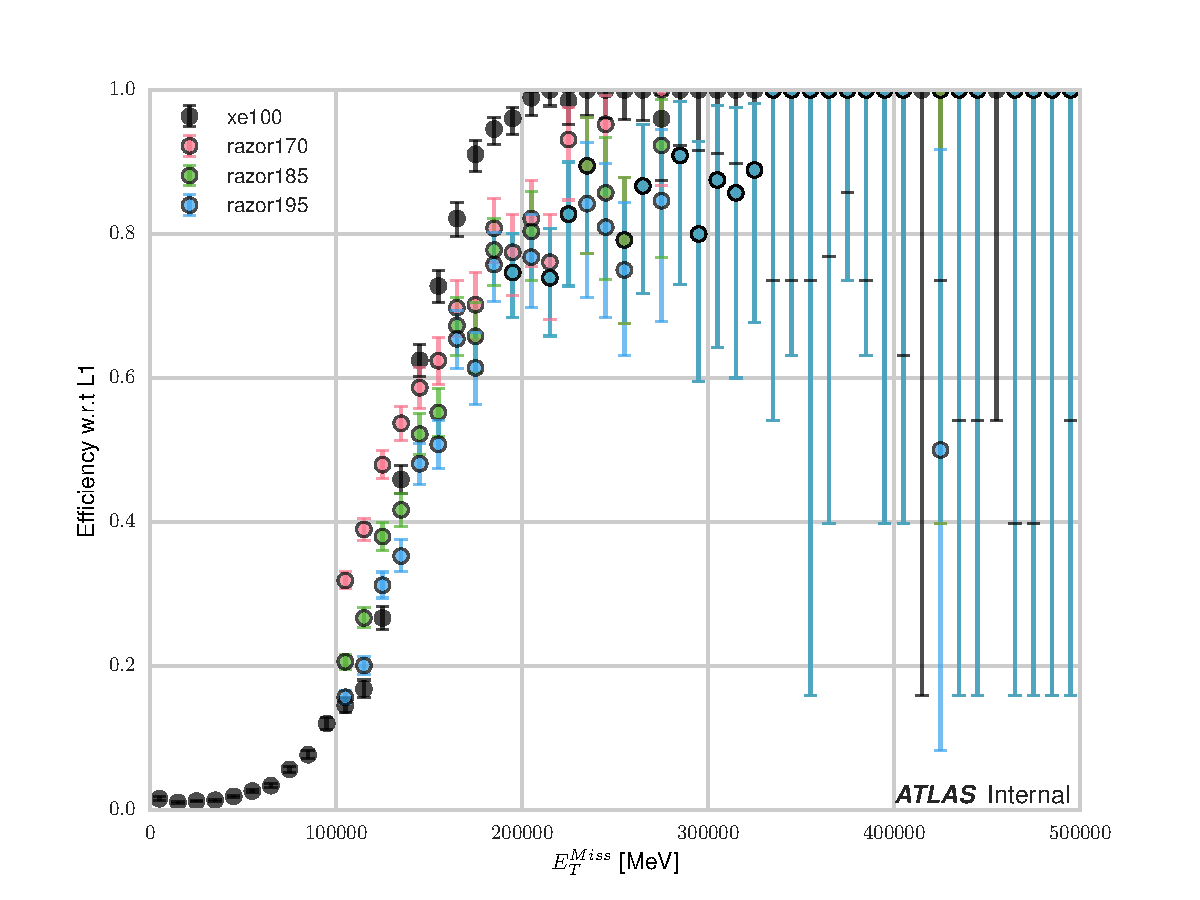
\includegraphics[width=.9\linewidth]{TurnOn_Met}\\
% 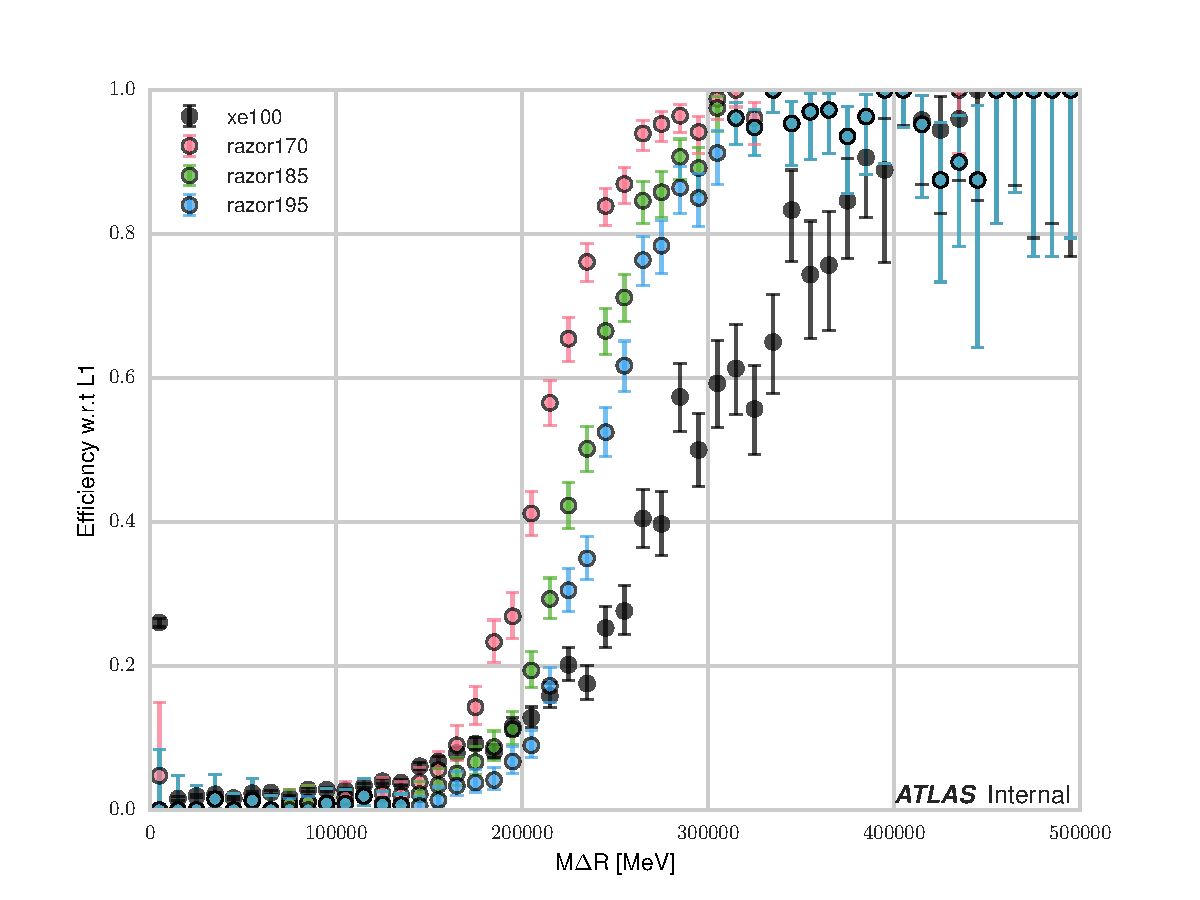
\includegraphics[width=.9\linewidth]{TurnOn_MDR}
% \end{figure}

% There was a quite big change in the 2016 menu, which increased the rate given to \met triggers drastically.
% This can be seen in the difference in rate shown between \met triggers in 2015 and 2016 in \Cref{tab:triggers}.
% This allowed the \met triggers to maintain a lower threshold throughout the dataset used in this thesis.
